% Options for packages loaded elsewhere
\PassOptionsToPackage{unicode}{hyperref}
\PassOptionsToPackage{hyphens}{url}
%
\documentclass[
]{book}
\usepackage{amsmath,amssymb}
\usepackage{iftex}
\ifPDFTeX
  \usepackage[T1]{fontenc}
  \usepackage[utf8]{inputenc}
  \usepackage{textcomp} % provide euro and other symbols
\else % if luatex or xetex
  \usepackage{unicode-math} % this also loads fontspec
  \defaultfontfeatures{Scale=MatchLowercase}
  \defaultfontfeatures[\rmfamily]{Ligatures=TeX,Scale=1}
\fi
\usepackage{lmodern}
\ifPDFTeX\else
  % xetex/luatex font selection
\fi
% Use upquote if available, for straight quotes in verbatim environments
\IfFileExists{upquote.sty}{\usepackage{upquote}}{}
\IfFileExists{microtype.sty}{% use microtype if available
  \usepackage[]{microtype}
  \UseMicrotypeSet[protrusion]{basicmath} % disable protrusion for tt fonts
}{}
\makeatletter
\@ifundefined{KOMAClassName}{% if non-KOMA class
  \IfFileExists{parskip.sty}{%
    \usepackage{parskip}
  }{% else
    \setlength{\parindent}{0pt}
    \setlength{\parskip}{6pt plus 2pt minus 1pt}}
}{% if KOMA class
  \KOMAoptions{parskip=half}}
\makeatother
\usepackage{xcolor}
\usepackage{longtable,booktabs,array}
\usepackage{calc} % for calculating minipage widths
% Correct order of tables after \paragraph or \subparagraph
\usepackage{etoolbox}
\makeatletter
\patchcmd\longtable{\par}{\if@noskipsec\mbox{}\fi\par}{}{}
\makeatother
% Allow footnotes in longtable head/foot
\IfFileExists{footnotehyper.sty}{\usepackage{footnotehyper}}{\usepackage{footnote}}
\makesavenoteenv{longtable}
\usepackage{graphicx}
\makeatletter
\newsavebox\pandoc@box
\newcommand*\pandocbounded[1]{% scales image to fit in text height/width
  \sbox\pandoc@box{#1}%
  \Gscale@div\@tempa{\textheight}{\dimexpr\ht\pandoc@box+\dp\pandoc@box\relax}%
  \Gscale@div\@tempb{\linewidth}{\wd\pandoc@box}%
  \ifdim\@tempb\p@<\@tempa\p@\let\@tempa\@tempb\fi% select the smaller of both
  \ifdim\@tempa\p@<\p@\scalebox{\@tempa}{\usebox\pandoc@box}%
  \else\usebox{\pandoc@box}%
  \fi%
}
% Set default figure placement to htbp
\def\fps@figure{htbp}
\makeatother
\setlength{\emergencystretch}{3em} % prevent overfull lines
\providecommand{\tightlist}{%
  \setlength{\itemsep}{0pt}\setlength{\parskip}{0pt}}
\setcounter{secnumdepth}{5}
\usepackage{booktabs}
\usepackage[]{natbib}
\bibliographystyle{plainnat}
\usepackage{bookmark}
\IfFileExists{xurl.sty}{\usepackage{xurl}}{} % add URL line breaks if available
\urlstyle{same}
\hypersetup{
  pdftitle={Quality Control Pipeline for Massively Parallel Reporter Assays (MPRAs)},
  pdfauthor={Omer Ronen},
  hidelinks,
  pdfcreator={LaTeX via pandoc}}

\title{Quality Control Pipeline for Massively Parallel Reporter Assays (MPRAs)}
\author{Omer Ronen}
\date{2025-09-30}

\begin{document}
\maketitle

{
\setcounter{tocdepth}{1}
\tableofcontents
}
\chapter*{Overview}\label{overview}
\addcontentsline{toc}{chapter}{Overview}

This pipeline is designed to help investigators evaluate the quality of their MPRA, quickly identify pitfalls, trace them to their source, and mitigate them. The scripts provided help ensure that the resulting MPRA data are suitable for robust statistical analysis and meaningful biological interpretation.
This Bookdown accompanies our guide for best practices for MPRAs, which outlines recommendations for study design and interpretation {[}REF{]}. The manuscript covers all key experimental and analytical steps, including library design, and estimation of activity differential activity. It then describes core problems that often compromise MPRA quality, illustrating how these issues manifest in the data, and offering practical strategies for correction and optimization.
Because each issue can influence multiple quality metrics, and each metric may be affected by several issues, the relationships form a many-to-many network. The figures presented below map these interdependencies and connect them to recommended diagnostic analyses.

\section*{Usage}\label{usage}
\addcontentsline{toc}{section}{Usage}

\pandocbounded{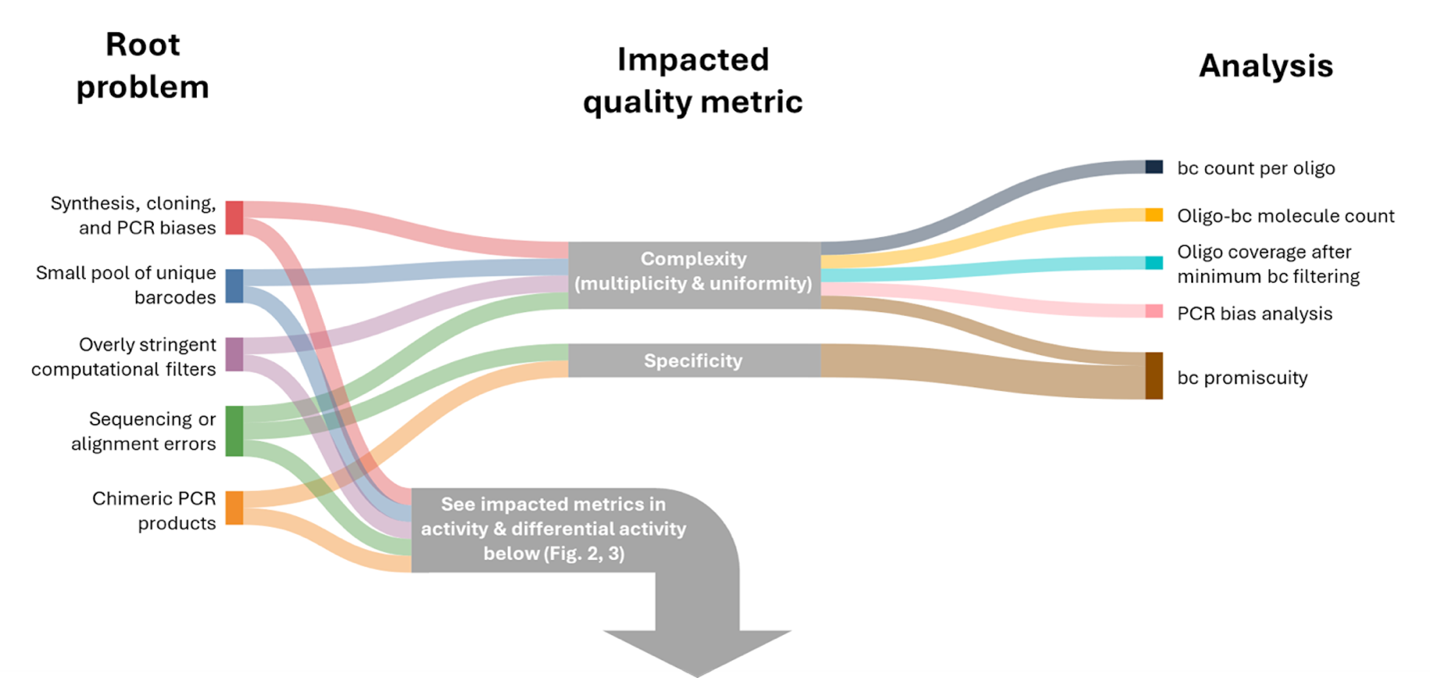
\includegraphics[keepaspectratio]{associations_root.png}}
A scheme of root problems, the impacted quality metrics and analyses for the cCRE-barcode association step.

\pandocbounded{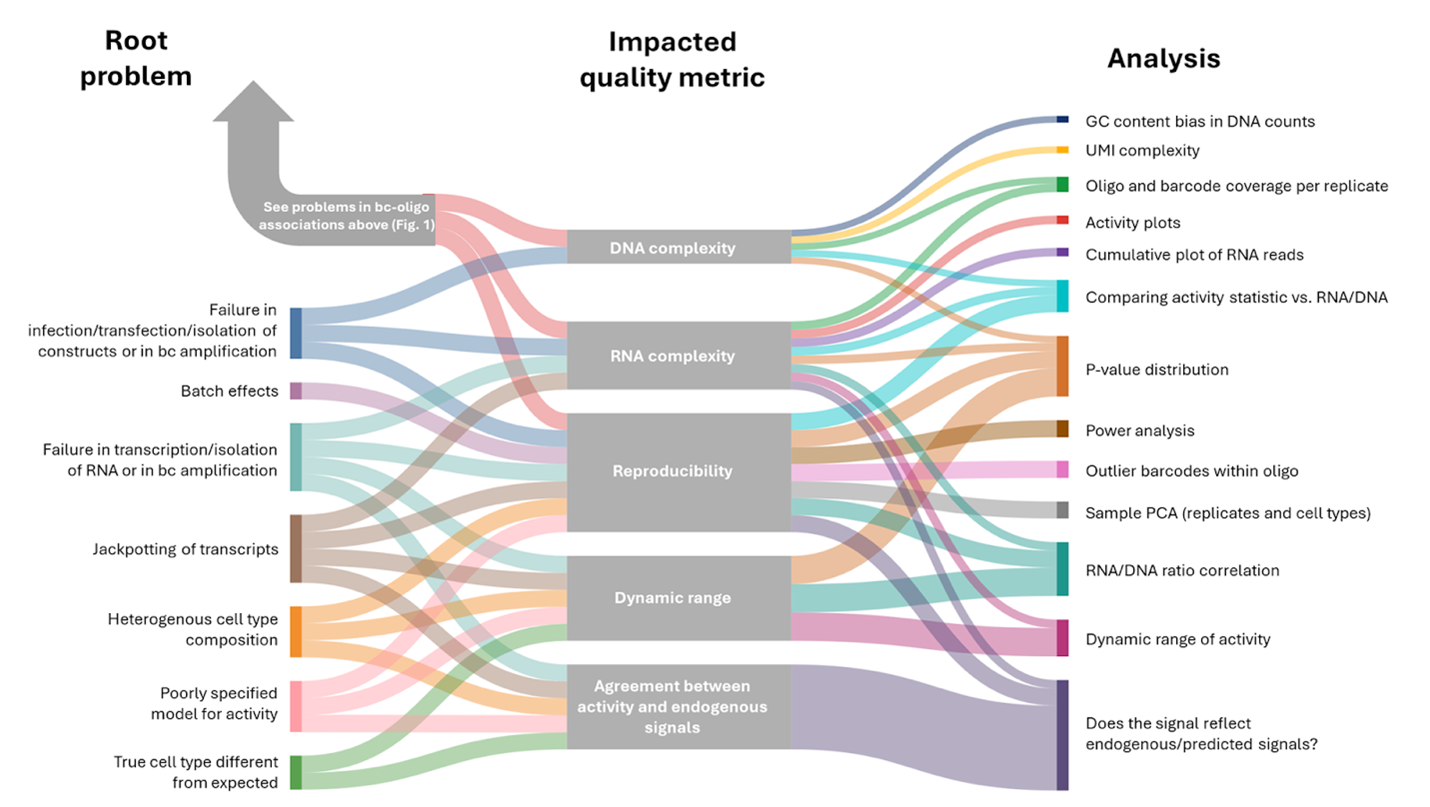
\includegraphics[keepaspectratio]{activity_root.png}}
Root problems, impacted quality metrics and recommended analyses for the RNA and DNA quantification step.

The quality control (QC) pipeline is organized into three chapters:

\begin{itemize}
\tightlist
\item
  \begin{enumerate}
  \def\labelenumi{(\roman{enumi})}
  \tightlist
  \item
    QC of the barcode association step\\
  \end{enumerate}
\item
  \begin{enumerate}
  \def\labelenumi{(\roman{enumi})}
  \setcounter{enumi}{1}
  \tightlist
  \item
    QC of activity estimation\\
  \end{enumerate}
\item
  \begin{enumerate}
  \def\labelenumi{(\roman{enumi})}
  \setcounter{enumi}{2}
  \tightlist
  \item
    QC of differential activity estimation
  \end{enumerate}
\end{itemize}

For each analysis, we provide an example of a successful and an unsuccessful dataset to illustrate how they manifest in the analysis.

We welcome questions, feedback, or suggestions. Please feel free to reach out at david.gokhman {[}at{]} weizmann.ac.il.

\section*{Scripts}\label{scripts}
\addcontentsline{toc}{section}{Scripts}

All of these analyses are integrated into the quality control pipeline described in this resource, with scripts provided here: {[}link{]}.

\chapter{A guide for running the analyses notebook}\label{a-guide-for-running-the-analyses-notebook}

The QC pipeline has three main parts: Associations, Activity and Differential activity.
For each part, there is a jupyter notebook file that enables you to run all the analyses that are presented in this book.
Here we explain how to run these notebook files and what are the required inputs

\section{Associations}\label{associations}

First

\subsection{Input}\label{input}

Input files

\section{Activity}\label{activity}

Second

\subsection{Input}\label{input-1}

Input files

\section{Differential Activity}\label{differential-activity}

Third

\subsection{Input}\label{input-2}

Input files

\chapter{Associations QC}\label{associations-qc}

\section{Barcodes per cCRE}\label{barcodes-per-ccre}

\textbf{Goal:}
\textbf{Input file:}
\textbf{Evaluated metrics}:

\pandocbounded{\includegraphics[keepaspectratio]{11-only_figs_associations_files/figure-latex/unnamed-chunk-3-1.pdf}}

\textbf{Legend:}
\textbf{Interpretation:}

\section{PCR bias - GC content}\label{pcr-bias---gc-content}

\subsection{Reads per GC bin}\label{reads-per-gc-bin}

\textbf{Goal:}
\textbf{Input file:}
\textbf{Evaluated metrics}:
\pandocbounded{\includegraphics[keepaspectratio]{11-only_figs_associations_files/figure-latex/unnamed-chunk-4-1.pdf}}

\textbf{Legend:}
\textbf{Interpretation:}

\subsection{cCRE counts}\label{ccre-counts}

\textbf{Goal:}
\textbf{Input file:}
\textbf{Evaluated metrics}:

\pandocbounded{\includegraphics[keepaspectratio]{11-only_figs_associations_files/figure-latex/unnamed-chunk-5-1.pdf}}

\textbf{Legend:}
\textbf{Interpretation:}

\section{PCR bias - G Stretch}\label{pcr-bias---g-stretch}

\subsection{Reads per G stretch bin}\label{reads-per-g-stretch-bin}

\textbf{Goal:}
\textbf{Input file:}
\textbf{Evaluated metrics}:

\pandocbounded{\includegraphics[keepaspectratio]{11-only_figs_associations_files/figure-latex/unnamed-chunk-6-1.pdf}}

\textbf{Legend:}
\textbf{Interpretation:}

\subsection{cCRE counts}\label{ccre-counts-1}

\textbf{Goal:}
\textbf{Input file:}
\textbf{Evaluated metrics}:
\pandocbounded{\includegraphics[keepaspectratio]{11-only_figs_associations_files/figure-latex/unnamed-chunk-7-1.pdf}}

\textbf{Legend:}
\textbf{Interpretation:}

\section{cCRE-barcode observations}\label{ccre-barcode-observations}

\textbf{Goal:}
\textbf{Input file:}
\textbf{Evaluated metrics}:
\pandocbounded{\includegraphics[keepaspectratio]{11-only_figs_associations_files/figure-latex/unnamed-chunk-8-1.pdf}}

\textbf{Legend:}
\textbf{Interpretation:}

\section{Retained cCREs}\label{retained-ccres}

\textbf{Goal:}
\textbf{Input file:}
\textbf{Evaluated metrics}:
\pandocbounded{\includegraphics[keepaspectratio]{11-only_figs_associations_files/figure-latex/unnamed-chunk-9-1.pdf}}

\textbf{Legend:}
\textbf{Interpretation:}

\section{Barcode promiscuity}\label{barcode-promiscuity}

\textbf{Goal:}
\textbf{Input file:}
\textbf{Evaluated metrics}:
\pandocbounded{\includegraphics[keepaspectratio]{11-only_figs_associations_files/figure-latex/unnamed-chunk-10-1.pdf}}

\textbf{Legend:}
\textbf{Interpretation:}

\section{Downsampling - Retained cCREs}\label{downsampling---retained-ccres}

\textbf{Goal:}
\textbf{Input file:}
\textbf{Evaluated metrics}:
\pandocbounded{\includegraphics[keepaspectratio]{11-only_figs_associations_files/figure-latex/unnamed-chunk-11-1.pdf}}

\textbf{Legend:}
\textbf{Interpretation:}

\section{Downsampling - Barcodes per cCRE}\label{downsampling---barcodes-per-ccre}

\textbf{Goal:}
\textbf{Input file:}
\textbf{Evaluated metrics}:
\pandocbounded{\includegraphics[keepaspectratio]{11-only_figs_associations_files/figure-latex/unnamed-chunk-12-1.pdf}}

\textbf{Legend:}
\textbf{Interpretation:}

\chapter{Activity QC}\label{activity-qc}

\section{Evaluating DNA and RNA complexity}\label{evaluating-dna-and-rna-complexity}

\subsection{Retained cCREs and barcodes}\label{retained-ccres-and-barcodes}

\textbf{Goal:}
\textbf{Input file:}
\textbf{Evaluated metrics}:

\begin{verbatim}
## Good example: PMID_38766054_Reilly 
## Bad example: Max_MPRA_run2
\end{verbatim}

\pandocbounded{\includegraphics[keepaspectratio]{12-only_figs_activity_files/figure-latex/unnamed-chunk-3-1.pdf}}
\textbf{Legend:}
\textbf{Interpretation:}

\subsection{Activity distribution}\label{activity-distribution}

\textbf{Goal:}
\textbf{Input file:}
\textbf{Evaluated metrics}:

\begin{verbatim}
## Good example: PMID_38766054_Reilly 
## Bad example: humanMPRA_L4a2 
## Bad example 2: humanMPRA_L1a1_Neurons
\end{verbatim}

\pandocbounded{\includegraphics[keepaspectratio]{12-only_figs_activity_files/figure-latex/unnamed-chunk-4-1.pdf}}

\begin{verbatim}
## [1] "add arrows that indicate right tail, symmetry, or no activity detected"
\end{verbatim}

\textbf{Legend:}
\textbf{Interpretation:}

\subsection{P-value distribution}\label{p-value-distribution}

\textbf{Goal:}
\textbf{Input file:}
\textbf{Evaluated metrics}:

Problem: nothitng looks mildly bad, max looks too bad.

\begin{verbatim}
## Good example: PMID_38766054_Reilly 
## Bad example: humanMPRA_L4a2
\end{verbatim}

\pandocbounded{\includegraphics[keepaspectratio]{12-only_figs_activity_files/figure-latex/unnamed-chunk-5-1.pdf}}
\textbf{Legend:}
\textbf{Interpretation:}

\subsection{Downsampling analysis - active cCREs}\label{downsampling-analysis---active-ccres}

\textbf{Goal:}
\textbf{Input file:}
\textbf{Evaluated metrics}:

we should use a real downsampling - Omer is in charge of that. In the bookdown we need to mention Max's script.
for Max's script - we should ask why there's a jump between the last and one-before-last downsampling. send him an email.
Also ask what does ``LP complexity'' mean in his script.

\pandocbounded{\includegraphics[keepaspectratio]{12-only_figs_activity_files/figure-latex/unnamed-chunk-6-1.pdf}}
\textbf{Legend:}
\textbf{Interpretation:}

\subsection{Cumulative RNA reads}\label{cumulative-rna-reads}

\textbf{Goal:}
\textbf{Input file:}
\textbf{Evaluated metrics}:

Add arrows in the x axis and below it ``decreasing RNA reads'' in illustrator.

\begin{verbatim}
## Good example: PMID_38766054_Reilly 
## Bad example: d2Osteoblast_spiking_oligos
\end{verbatim}

\pandocbounded{\includegraphics[keepaspectratio]{12-only_figs_activity_files/figure-latex/unnamed-chunk-7-1.pdf}}
\textbf{Legend:}
\textbf{Interpretation:}

\section{Evaluating reproducibility}\label{evaluating-reproducibility}

\subsection{Similarity between samples (PCA)}\label{similarity-between-samples-pca}

\textbf{Goal:}
\textbf{Input file:}
\textbf{Evaluated metrics}:

mention in the bookdown: the importance of the percentage explained by the 1st and 2nd PCs.

\begin{verbatim}
## Good example: PMID_38766054_Reilly 
## Bad example: thylacine_biorxiv_Gallego_Romero
\end{verbatim}

\pandocbounded{\includegraphics[keepaspectratio]{12-only_figs_activity_files/figure-latex/unnamed-chunk-8-1.pdf}}
\textbf{Legend:}
\textbf{Interpretation:}

\subsection{Correlation between replicates}\label{correlation-between-replicates}

\textbf{Goal:}
\textbf{Input file:}
\textbf{Evaluated metrics}:

\begin{verbatim}
## Good example: thylacine_biorxiv_Gallego_Romero 
## Bad example: humanMPRA_L4a2
\end{verbatim}

\pandocbounded{\includegraphics[keepaspectratio]{12-only_figs_activity_files/figure-latex/unnamed-chunk-9-1.pdf}}

\begin{verbatim}
## Warning in rm(good_example_MPRA, bad_example_MPRA, bad_example_MPRA_2,
## analysis_name): object 'bad_example_MPRA_2' not found
\end{verbatim}

\textbf{Legend:}
\textbf{Interpretation:}

\subsection{Variation at various activity levels}\label{variation-at-various-activity-levels}

\textbf{Goal:}
\textbf{Input file:}
\textbf{Evaluated metrics}:

Omer is in charge of this part.

\pandocbounded{\includegraphics[keepaspectratio]{12-only_figs_activity_files/figure-latex/unnamed-chunk-10-1.pdf}}
\textbf{Legend:}
\textbf{Interpretation:}

\subsection{Correlation between replicates (controls)}\label{correlation-between-replicates-controls}

\textbf{Goal:}
\textbf{Input file:}
\textbf{Evaluated metrics}:

\begin{verbatim}
## Good example: PMID_38766054_Reilly 
## Bad example: Max_MPRA_run2
\end{verbatim}

\pandocbounded{\includegraphics[keepaspectratio]{12-only_figs_activity_files/figure-latex/unnamed-chunk-11-1.pdf}}
\textbf{Legend:}
\textbf{Interpretation:}

\subsection{RNA\_DNA\_ratio}\label{rna_dna_ratio}

\textbf{Goal:}
\textbf{Input file:}
\textbf{Evaluated metrics}:

\begin{verbatim}
## Good example: PMID_38766054_Reilly 
## Bad example: humanMPRA_L4a2 
## Bad example 2: humanMPRA_L1a1_Neurons
\end{verbatim}

\pandocbounded{\includegraphics[keepaspectratio]{12-only_figs_activity_files/figure-latex/unnamed-chunk-12-1.pdf}}
\textbf{Legend:}
\textbf{Interpretation:}

\subsection{Activity of controls - sample comparison}\label{activity-of-controls---sample-comparison}

\textbf{Goal:}
\textbf{Input file:}
\textbf{Evaluated metrics}:

\begin{verbatim}
## Good example: PMID_38766054_Reilly 
## Bad example: Max_MPRA_run2
\end{verbatim}

\pandocbounded{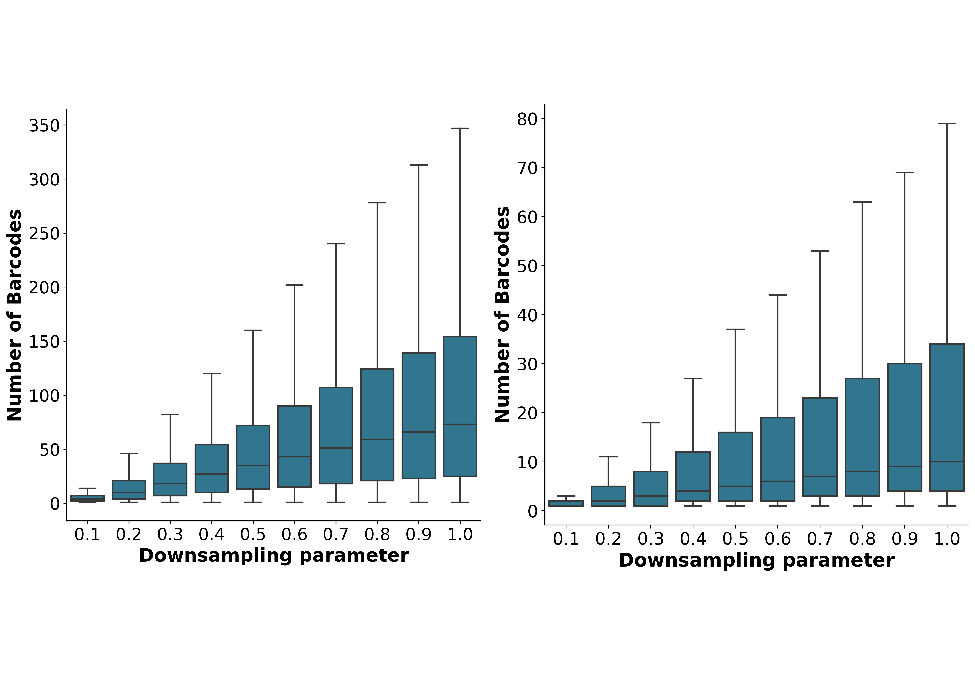
\includegraphics[keepaspectratio]{12-only_figs_activity_files/figure-latex/unnamed-chunk-13-1.pdf}}
\textbf{Legend:}
\textbf{Interpretation:}

\subsection{Minimizing noise {[}Outlier barcodes + min(DNA){]} - use the mhMPRA data}\label{minimizing-noise-outlier-barcodes-mindna---use-the-mhmpra-data}

\textbf{Goal:}
\textbf{Input file:}
\textbf{Evaluated metrics}:

\pandocbounded{
\includegraphics[keepaspectratio]{12-only_figs_activity_files/figure-latex/unnamed-chunk-14-1.pdf}}
\textbf{Legend:}
\textbf{Interpretation:}

\subsection{Outlier barcodes}\label{outlier-barcodes}

\textbf{Goal:}
\textbf{Input file:}
\textbf{Evaluated metrics}:

\pandocbounded{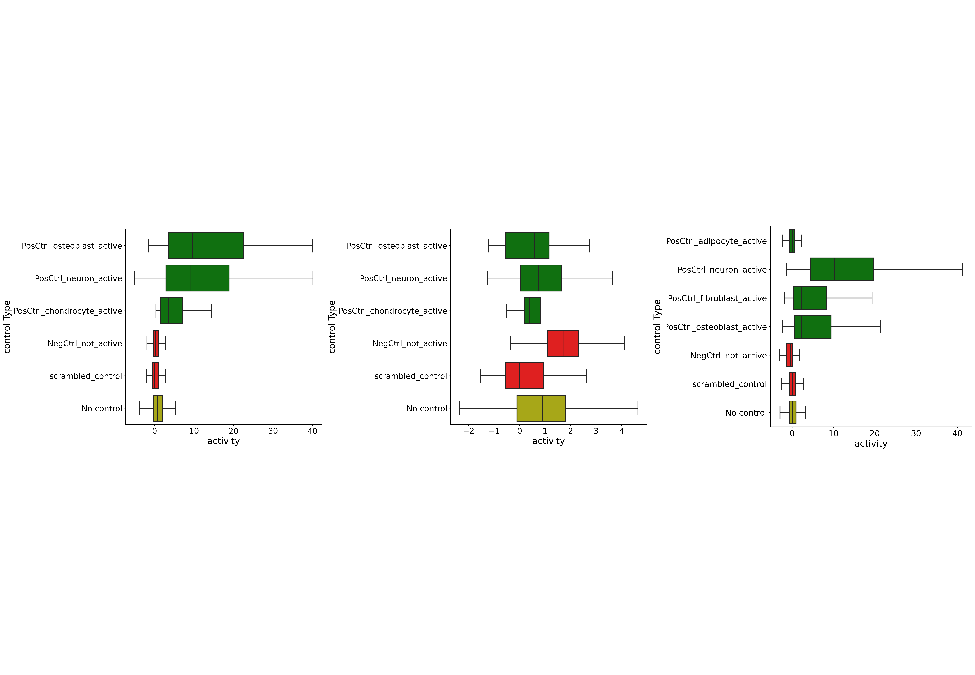
\includegraphics[keepaspectratio]{12-only_figs_activity_files/figure-latex/unnamed-chunk-15-1.pdf}}

  \bibliography{book.bib,packages.bib}

\end{document}
